\chapter{実装}
本章では、第2章で述べたシステムの設計を受け、Hyper Launcherの実装について述べる。

\newpage

\section{システム構成}
Hyper Launcherはユーザーがアプリケーションを登録するためのクライアントと、登録したデータを保存しておくためのデータストアから構成される。構成図を図\ref{fig:system}に示す。

\begin{figure}[h]
    \begin{center}
       \fbox{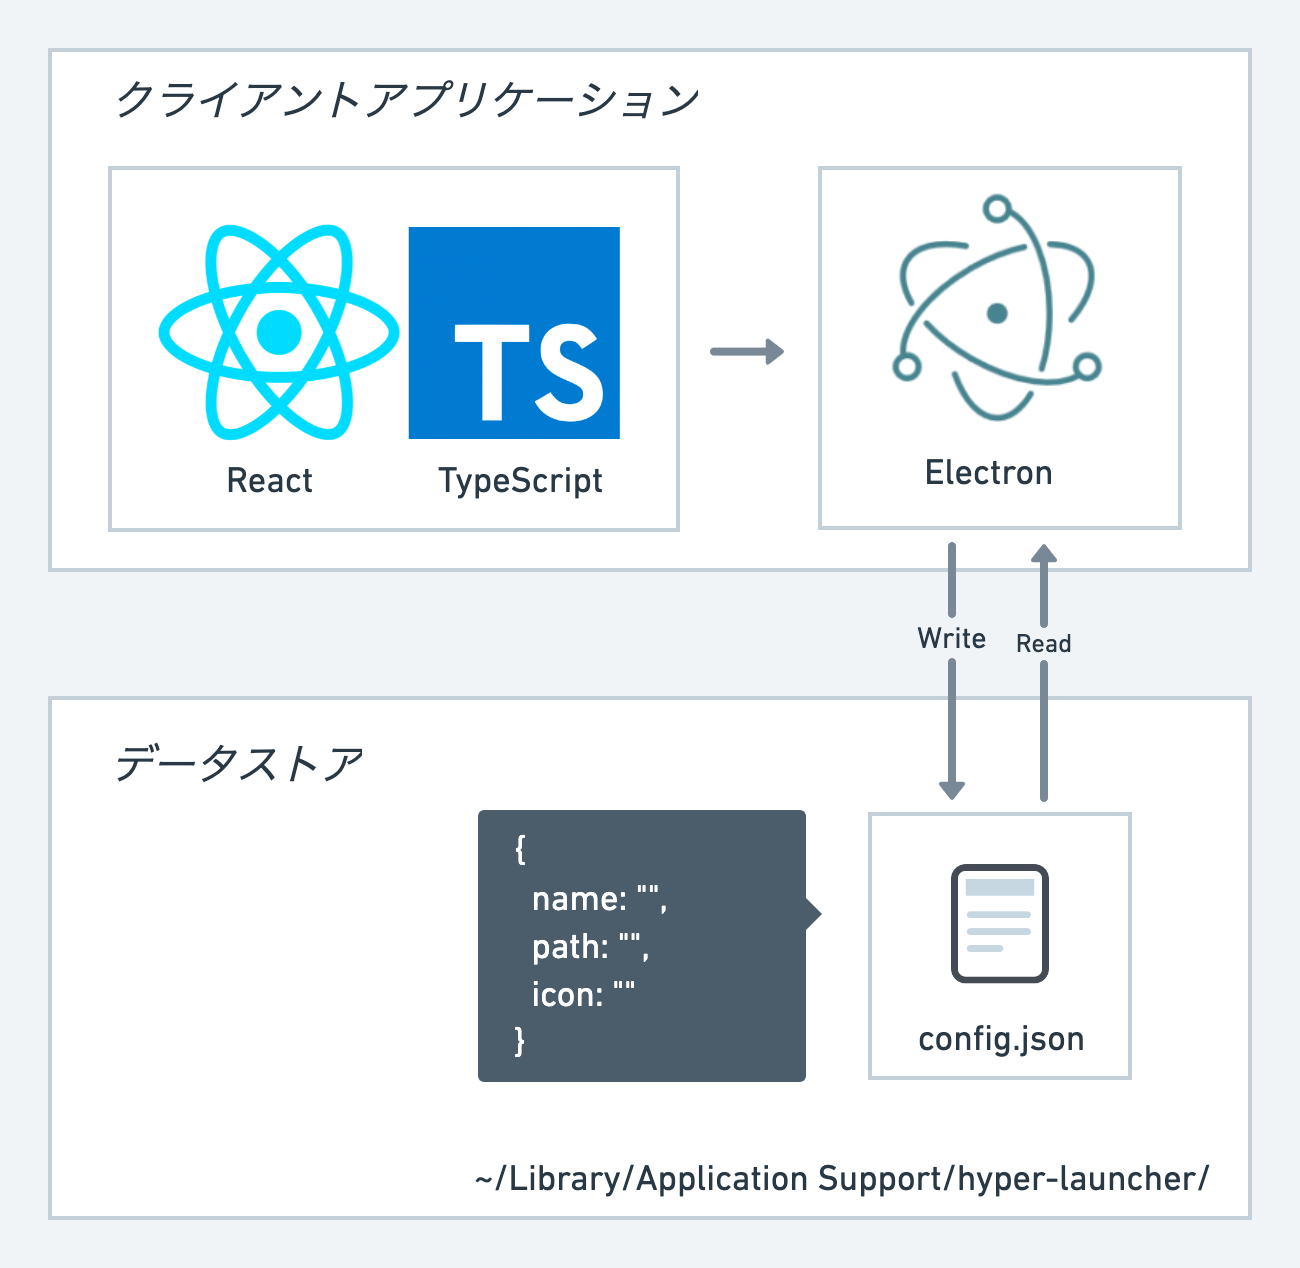
\includegraphics[width=100mm]{images/system}}
    \end{center}
    \caption{システムの構成}
    \label{fig:system}
\end{figure}

\section{クライアント}
クライアントはElectron\footnote{https://electronjs.org}やTypeScript\footnote{https://www.typescriptlang.org/}、React\footnote{https://reactjs.org}といったWeb技術によって実装されており、macOSのデスクトップアプリケーションとして動作する。

\subsubsection{Electron}
ElectronはHTML、JavaScript、CSSを用いてクロスプラットフォームなデスクトプアプリケーションを作成することができるソフトウェアフレームワークである。Electron自体はChromiumとNode.jsを使用しておりWeb技術のみで開発が完結するのが利点である。Hyper LauncherではElectronのglobalShortcutというAPIを利用し、Hyper Launcherが非アクティブ状態でもホットキーの入力を取得できるようになっている。アプリケーションの起動やアクティブ化なども標準の機能だけで実装できるため、ランチャーに適したフレームワークと言える。

\subsubsection{AppleScript}
Web技術のみでは実装が難しい部分についてはAppleScriptを使用した。masOSにはosascriptと呼ばれるシェルスクリプトが存在し、これを利用することでNode.js\footnote{https://nodejs.org}からAppleScriptを実行することができる。AppleScriptによって、起動中のアプリケーションや特定のアプリケーションがアクティブかどうかといった情報を取得することができ、これによってデスクトップアプリケーションとして十分な機能を実装することが可能となった。ただし実行する毎にプロセスを立ち上げるため、無闇に使用してしまうとラグが発生してしまう。また、AppleScriptはmacOSのみで使えるものであるため、Electronの利点であるクロスプラットフォーム対応はできなくなってしまった。

\section{データストア}
ユーザーが登録した情報は、Electronが定義するユーザーデータ領域(~/Library/Application Support/hyper-launcher/)にJSONファイルとして保存されている。データのやり取りが全てローカルで完結するため、オフラインでも使用できようになっている。データはホットキーの数字をキーにしアプリケーション情報の配列を値として持ったオブジェクトになっており、アプリケーション情報にはアプリケーションの名前、パス、そしてbase64エンコードされたアイコンの3つが含まれている。これにより単一のキーに対して複数のアプリケーションを登録することが可能となっている。以下にその例を示す。ただしiconのbase64文字列と中間部分は長くなるため省略した。

\begin{lstlisting}[caption=config.json]
{
  "shortcut": {
    "1": [
      {
        "name": "ForkLift",
        "path": "/Applications/ForkLift.app",
        "icon": "***************************"
      }
    ],
    "2": [
      {
        "name": "Hyper",
        "path": "/Applications/Hyper.app",
        "icon": "***************************"
      }
    ],
    
    ・・・
    
    "9": [
      {
        "name": "Hyper Launcher",
        "path": "/Applications/Hyper Launcher.app",
        "icon": "***************************"
      }
    ],
  }
}
\end{lstlisting}